\section*{Задача 6.2}
\subsection*{Постановка задачи}
Найти приближенное решение задачи Коши для обыкновенного дифференциального уравнения (ОДУ) 1-го порядка с точностью $\varepsilon = 10^{-6}$ на отрезке $[\pi/2, \pi/2 + 0.8]$.
\[
	\begin{cases}
		y' = -\dfrac{y}{t} + \dfrac{\cos{t}}{t} \\
		y(\pi/2) = 0
	\end{cases}
\]
\subsection*{Решение}
Найдем аналитическое решение:
\begin{gather*}
	y' + \dfrac{y}{t} = 0 \\
	y_{одн} = \dfrac{C(t)}{t}\\
	y_{одн}' = \dfrac{tC'(t) - C(t)}{t^2}\\
	y_{одн}' + \dfrac{y_{одн}}{t} = \dfrac{C'(t)}{t} - \dfrac{C(t)}{t^2} + \dfrac{C(t)}{t^2} = \dfrac{\cos{t}}{t} \\
	C'(t) = \cos{t} \\
	y = \dfrac{\sin{t}}{t} + \dfrac{C}{t}\\
	y = \dfrac{\sin{t}}{t} - \dfrac{1}{t}
\end{gather*}

Запишем расчетную формулу для метода Эйлера: $y_{i+1} = y_i + hf(t_i, y_i)$ и правило Рунге для данного метода: $y^{h/2}_i - y(t_i) \approx y^{h/2}_i - y^{h}_i$. При поиске решения с точностью $\varepsilon = 10^{-6}$ с помощью данного метода потребовалось 131073 точки, то есть шаг, на котором точность достигается равен $h = 6.103515625 \times 10^{-6}$.

При поиске решения с помощью экстраполяционного метода Адамса 3-го порядка, так как нам известно точное решение, зададим значения в точках $y_1 = y(a + h), y_2 = y(a + 2h)$ так как метод является 3-х точечным. Ниже представлена  расчетная формула данного метода. Для нахождения решения с заданной точностью потребовалось 65 точек, то есть величина шага составила $h = 0.0125$.
\[
	y_{i+1} = y_i + \dfrac{h}{12}[23f(t_i, y_i) - 16f(t_{i-1}, y_{i-1}) + 5f(t_{i-2}, y_{i-2})]
\]

Ниже на графиках представлены графики точного и приближенного решений, а также графики погрешностей.

\begin{figure}[h!]
	\centering                                                                                            
	\begin{minipage}{0.45\textwidth}
	        \centering
	        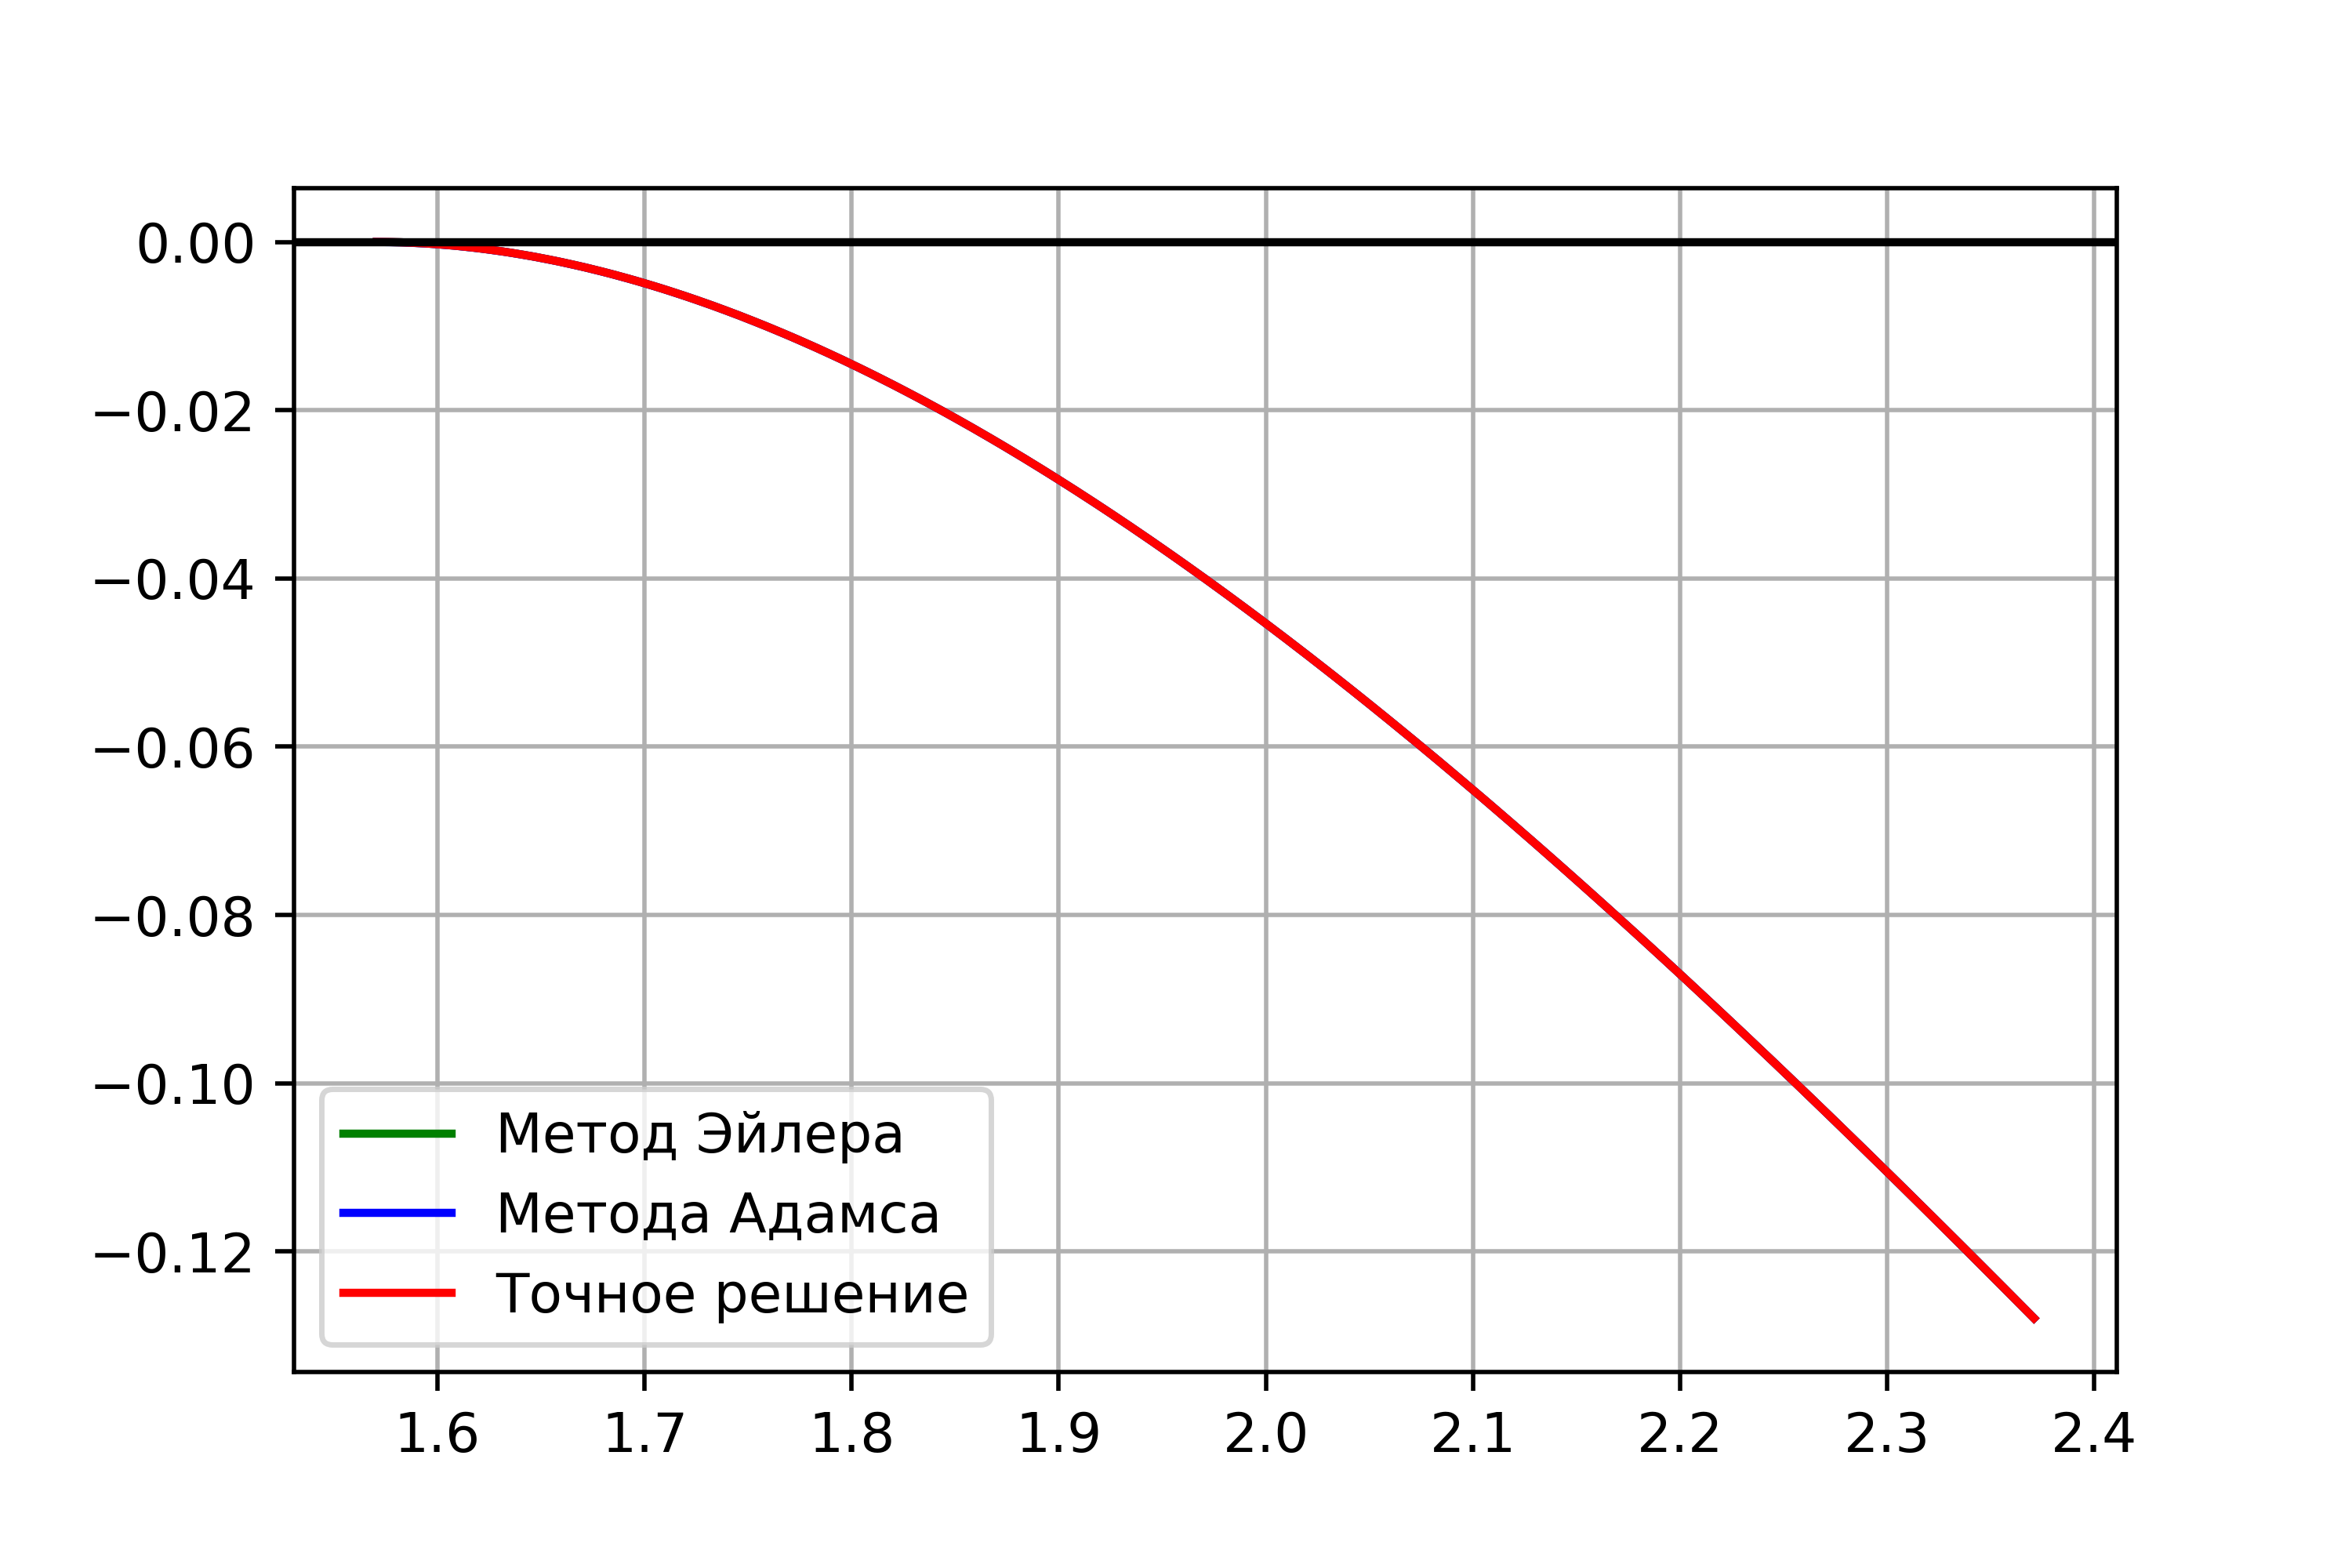
\includegraphics[width=8.5cm]{images/6.2_solution_plot.png} % первое изображение
	        \caption{Графики решений}
	\end{minipage}\hfill
	\begin{minipage}{0.45\textwidth}
		\centering
		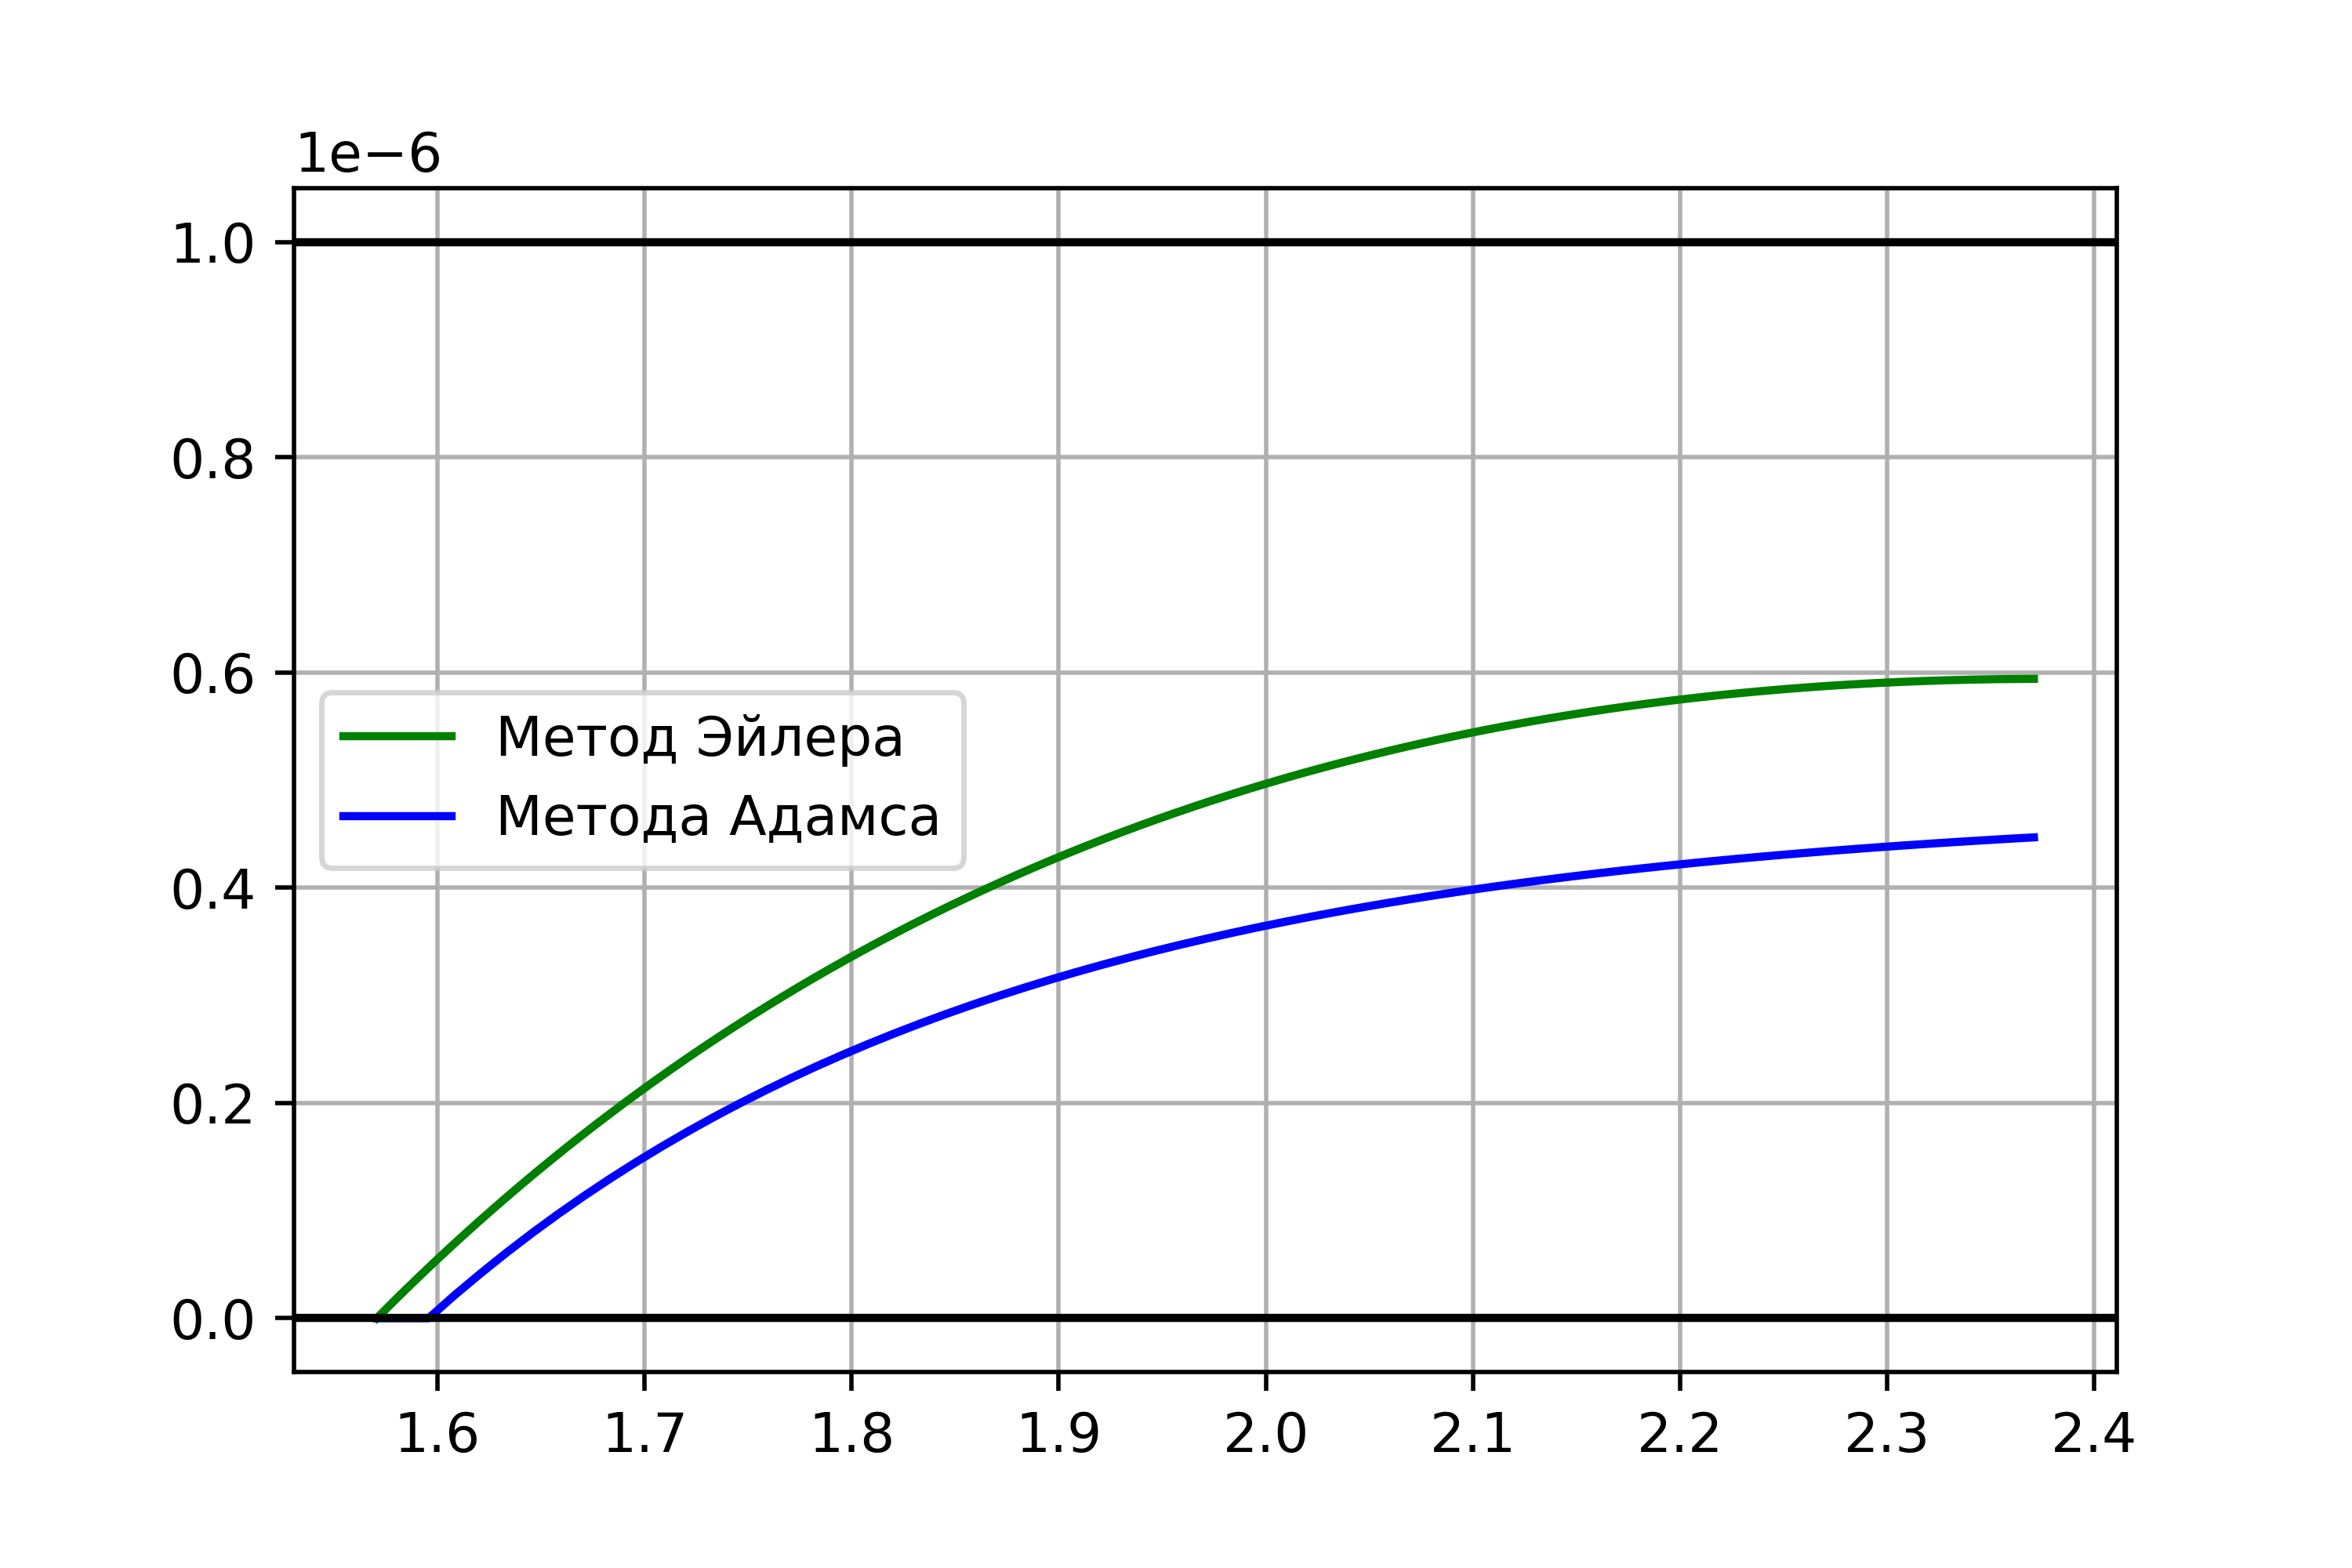
\includegraphics[width=8.5cm]{images/6.2_solution_err_plot.png} % второе изображение
		\caption{Погрешность нахождения решений}
	\end{minipage}
\end{figure}

На втором графике(Рис. 6) Видно, что метод Адамса показывает большую точность, причем на меньшем количестве узлов, что является результатом более высокого порядка точности данного метода по сравнению с методом Эйлера.